\documentclass[12pt]{article}

\usepackage{lmodern}
\usepackage[T1]{fontenc}
\usepackage[utf8]{inputenc}
\usepackage[spanish]{babel}
\usepackage{amsmath}
\usepackage{graphicx}
\usepackage[colorlinks=true, allcolors=blue]{hyperref}
\title{Práctica 2}
\author{Iván López Cervantes}
\date{}
\begin{document}
\maketitle
\section*{Ejercicio 1}
\subsection*{Enunciado}
Lenguaje sobre el alfabeto \{a, b\} que sólo contiene la cadena a.
\subsection*{Solución}
Autómata finito determinista generado:
$(\{q0, q1, q2\},\{a, b\}, \delta, q0, \{q2\})$
\begin{equation*}
\delta(q0, a) = q2 \hspace{1cm} \delta(q0, b) = q1
\end{equation*}
\begin{equation*}
\delta(q1, a) = q1 \hspace{1cm} \delta(q1, b) = q1
\end{equation*}
\begin{equation*}
\delta(q2, a) = q2 \hspace{1cm} \delta(q2, b) = q1
\end{equation*}
\begin{figure}[h]
    \centering
    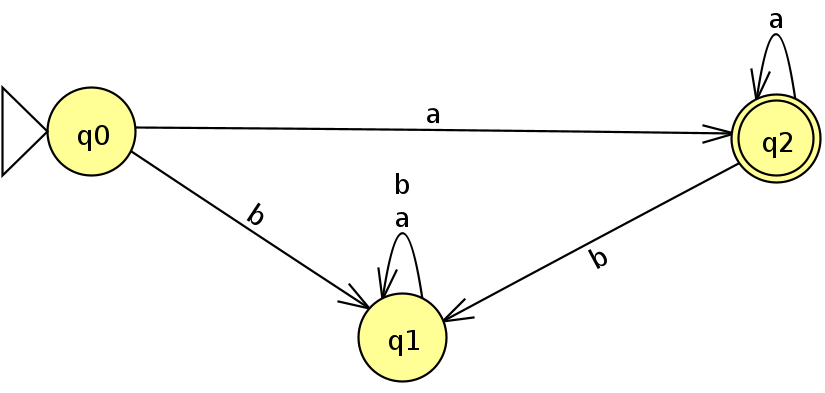
\includegraphics[scale=0.5]{DFA.png}
\end{figure}

\section*{Ejercicio 2}
\subsection*{Enunciado}
Introduce el autómata del ejercicio anterior en \textbf{finiteautomata.json}
\subsection*{Solución}
Texto en json: 
\begin{verbatim}
[
    {
        "name" : "only_a",
        "representation" : {
        "K" : ["q0", "q1", "q2"],
        "A" : ["a", "b"],
        "s" : "q0",
        "F" : ["q1"],
        "t" : [["q0", "a", "q2"],
                ["q0", "b", "q1"],
                ["q1", "a", "q1"],
                ["q1", "b", "q1"],
                ["q2", "a", "q2"],
                ["q2", "b", "q1"]]
        }
    }
]
\end{verbatim}

\end{document}
